% In the appendix, single-column tables may be set where they occur instead of being queued to column tops.
\makeatletter\renewcommand{\fps@table}{!htb}\makeatother

\section{Benchmark details}
\label{app:bench}

\paragraph{Fault operators}
Table~\ref{tab:ops} lists the operators. Each is applied to a gold formula; the result is kept as a fault only if the independent engine returns an error or a different value. Circular classes are generated at the position where users make them: the totals row under a numeric column, so the target cell lies inside the used column span. The \code{QUERY} class is generated from scratch and labelled by construction.

\begin{table}[t]
\caption{Fault operators and semantics-preserving variants used by \sheetfault.}
\label{tab:ops}
\centering\footnotesize
\begin{tabular}{>{\raggedright\arraybackslash}p{1.35cm} >{\raggedright\arraybackslash}p{2.75cm} >{\raggedright\arraybackslash}p{4.0cm}}
\toprule
\textbf{Group} & \textbf{Class} & \textbf{Operator} \\
\midrule
Structural & unbalanced parenthesis / quote & delete the final \code{)} / one \code{"} \\
 & missing \code{=} & drop the leading \code{=} \\
 & injection & append \code{+DDE("cmd|...")} or use a \code{HYPERLINK} to a \code{javascript:} URL \\
Symbols & hallucinated function & rename to a plausible invented name (\code{SUMIFF}, \code{COUNTWHERE}, \code{MEAN}, \code{NTHLARGEST}, \dots) \\
 & non-existent sheet & singular/plural variant, \code{Sheet2}, \code{Data}, \code{<name>\_old}, or prefix an own-sheet range with a missing sheet \\
 & column beyond data & move a range to a column 1--6 past the last used column \\
 & header used as name & replace a range by its column's header text (\code{=SUM(Revenue)}) \\
 & \code{QUERY} column OOB & select a column letter beyond the range's width \\
Shape & lookup index too large & \code{VLOOKUP} index = number of lookup columns + 3 \\
 & range size mismatch & shorten the last range of a multi-range function by 5--15 rows \\
Grounding & criterion absent & alter a string criterion (\code{"East"} $\to$ \code{"Easts"}, \code{"Northeast"}) \\
 & aggregate over text & replace the aggregated numeric range by a categorical column \\
Circularity & self reference & add the target cell to the formula \\
 & range / column contains self & totals-row range \code{F2:F81} or whole column \code{F:F} in \code{F81} \\
 & cycle via cell / range & the formula reads a helper cell whose formula reads the target cell / a range containing it \\
Semantic & wrong numeric column & swap one numeric range for another numeric column \\
 & wrong function & \code{SUM}$\leftrightarrow$\code{AVERAGE}, \code{MAX}$\leftrightarrow$\code{MIN}, \code{SUMIF}$\leftrightarrow$\code{AVERAGEIF}, \dots \\
\midrule
Benign variants & (negatives) & rows of headroom; absolute references; whole-column references; lowercase function names; extra spacing; own-sheet prefix; \code{IFERROR} wrapper; named range \\
\bottomrule
\end{tabular}
\end{table}

\paragraph{Task templates}
Fourteen templates: aggregate (\code{SUM/AVERAGE/MAX/MIN}), record count, conditional sum, conditional count, conditional average, two-condition \code{SUMIFS}/\code{COUNTIFS}, cross-sheet \code{VLOOKUP}, share of total, count above a threshold, \code{MAXIFS}, \code{SUMPRODUCT}, rounded average, $k$-th largest, and \code{INDEX/MATCH} for the row with the largest value. Each has an exact-header surface form (\emph{Sum Revenue where Region is East.}) and a paraphrase form (\emph{What is the total sales for the East territory?}) whose column mentions share no token with the headers.

\begin{table}
\caption{Share of clean formulas rejected or flagged, by class (\%). Every class is valid by construction or confirmed equivalent to the gold formula by the engine; custom functions cannot be checked and are only warned about.}
\label{tab:e1-clean}

\centering\footnotesize
\begin{adjustbox}{max width=\columnwidth}\begin{tabular}{l r rr rr}
\toprule
& & \multicolumn{2}{c}{\textbf{Shipped (v1)}} & \multicolumn{2}{c}{\textbf{\gc}} \\
\cmidrule(lr){3-4}\cmidrule(lr){5-6}
\textbf{Clean class} & n & Rej. & Flag & Rej. & Flag \\
\midrule
Gold formula & 864 & 0.0 & 15.3 & 0.0 & 0.0 \\
Rows of headroom & 396 & 0.0 & 100.0 & 0.0 & 0.0 \\
Absolute references & 783 & 0.0 & 16.9 & 0.0 & 0.0 \\
Whole-column references & 304 & 0.0 & 1.0 & 0.0 & 0.0 \\
Lowercase function names & 864 & 0.0 & 2.4 & 0.0 & 0.0 \\
Extra spacing & 751 & 0.0 & 17.6 & 0.0 & 0.0 \\
Own-sheet prefix & 783 & 0.0 & 16.9 & 0.0 & 0.0 \\
\code{IFERROR} wrapper & 864 & 0.0 & 15.3 & 0.0 & 0.0 \\
Named range & 99 & 0.0 & 19.2 & 0.0 & 0.0 \\
Ordinary totals-row formula & 864 & 0.0 & 0.0 & 0.0 & 0.0 \\
Valid \code{QUERY} & 144 & 0.0 & 0.0 & 0.0 & 0.0 \\
Handwritten valid syntax & 4{,}032 & 0.0 & 8.9 & 0.0 & 0.0 \\
Custom (non-Sheets) function & 144 & 0.0 & 100.0 & 0.0 & 100.0 \\
\bottomrule
\end{tabular}\end{adjustbox}
\end{table}


\section{Verifier details}
\label{app:verifier}

The function list holds 520 names: the 513 functions of the official Sheets list~\cite{googlefunctions} plus seven that exist but are missing from that table. The shipped list held 150 names and omitted 365 of the 513 official functions, including \code{PRODUCT}, \code{AVERAGEIF}, \code{AVERAGEIFS}, \code{MAXIFS}, \code{GEOMEAN} and \code{COUNTUNIQUE}. A function is a hard error only if it is within edit distance 2 of a known name (1 for names shorter than six characters). Arity entries cover about 90 functions; we compared them with the documented syntax and corrected two. The grounding layer reads at most 500 rows per referenced column and judges a column as categorical only if it was read completely or has at most 25 distinct values. Layer switches live in \code{CONFIG.VERIFICATION.LAYERS} and the repair policy in \code{CONFIG.VERIFICATION.REPAIR\_ON\_SUSPICIOUS}.

\section{Prompts}
\label{app:prompts}
The formula agent's system prompt is: \emph{``You are an expert Google Sheets formula engineer. [memory hints] RULES: 1. Output ONLY the raw formula starting with =. No markdown, no backticks, no explanation. 2. Use the spreadsheet context below to scope ranges correctly. 3. If data goes to row N, use that exact row number (not open-ended ranges unless appropriate). 4. Use the column letters and header names from the context. 5. If the user references a previous formula, check the conversation history.''} followed by three worked examples and the context block. After a failed verification the appended user turn has the form:
\begin{quote}\small\ttfamily
Your formula failed verification on attempt 2:\\
Formula: =SUM(Revenue)\\
HARD ERRORS (must fix):\\
\hspace*{1em}$\times$ "Revenue" is not a function, named range or cell reference.\\
CORRECTION HINTS:\\
\hspace*{1em}$\rightarrow$ "Revenue" is a column header (column D). Reference it by cell range, e.g. D2:D80, not by name.
\end{quote}

\section{Additional results}
\label{app:results}

\paragraph{Detection by fault class}
Table~\ref{tab:e1-classes} gives reject/flag recall for every fault class. \gc{} rejects every structural fault, every circular class, and the non-existent-sheet, header-as-name and lookup-index classes; where it only flags (criterion absent from its column, aggregation over a text column) this is the policy of Section~\ref{sec:gc}. The two semantic classes are valid formulas that answer the wrong question; the few hits in the last row coincide with the share of mutants that are loud.

\begin{table}
\caption{Recall per fault class, as reject/flag \%. \emph{Loud}: the independent engine returns an error value (the user would see it); otherwise the wrong formula evaluates silently to a plausible but wrong value. The two semantic classes are valid formulas that answer the wrong question; no verifier that cannot see the user's intent can reject them.}
\label{tab:e1-classes}

\centering\footnotesize
\begin{adjustbox}{max width=\columnwidth}\begin{tabular}{l c r ccc}
\toprule
\textbf{Fault class} & \textbf{Loud} & \textbf{n} & \textbf{Linter} & \textbf{Shipped} & \textbf{\gc} \\
\midrule
\multicolumn{6}{l}{\emph{Structural}} \\
~~Unbalanced parenthesis & yes &864 & 100/100 & 100/100 & \textbf{100/100} \\
~~Unbalanced quote & yes &581 & 100/100 & 100/100 & \textbf{100/100} \\
~~Missing \texttt{=} & no &864 & 100/100 & 100/100 & \textbf{100/100} \\
~~Injection (DDE/JS) & 54\% &864 & 54/54 & 100/100 & \textbf{100/100} \\
\addlinespace[2pt]
\multicolumn{6}{l}{\emph{Symbols}} \\
~~Hallucinated function & yes &864 & 100/100 & 0/100 & \textbf{64/100} \\
~~Non-existent sheet & yes &860 & 0/0 & 100/100 & \textbf{100/100} \\
~~Column beyond data & 43\% &772 & 0/0 & 0/100 & \textbf{97/97} \\
~~Header used as name & yes &783 & 0/0 & 0/17 & \textbf{100/100} \\
~~QUERY column out of range & yes &144 & 0/0 & 100/100 & \textbf{100/100} \\
\addlinespace[2pt]
\multicolumn{6}{l}{\emph{Shape}} \\
~~VLOOKUP index too large & yes &81 & 0/0 & 0/0 & \textbf{100/100} \\
~~Range size mismatch & yes &387 & 0/0 & 0/33 & \textbf{100/100} \\
\addlinespace[2pt]
\multicolumn{6}{l}{\emph{Grounding}} \\
~~Criterion absent from column & 30\% &505 & 0/0 & 0/23 & \textbf{0/100} \\
~~Aggregate over text column & 30\% &443 & 0/0 & 0/28 & \textbf{0/100} \\
\addlinespace[2pt]
\multicolumn{6}{l}{\emph{Circularity}} \\
~~Self reference & yes &864 & 0/0 & 100/100 & \textbf{100/100} \\
~~Range contains own cell & yes &864 & 0/0 & 0/100 & \textbf{100/100} \\
~~Whole column contains own cell & yes &864 & 0/0 & 0/0 & \textbf{100/100} \\
~~Cycle via other cell & yes &864 & 0/0 & 100/100 & \textbf{100/100} \\
~~Cycle via other range & yes &864 & 0/0 & 0/0 & \textbf{100/100} \\
\addlinespace[2pt]
\multicolumn{6}{l}{\emph{Semantic (undetectable by design)}} \\
~~Wrong numeric column & no &617 & 0/0 & 0/20 & \textbf{0/0} \\
~~Wrong aggregation function & 9\% &407 & 0/0 & 0/52 & \textbf{9/9} \\
\bottomrule
\end{tabular}\end{adjustbox}
\end{table}


\paragraph{Real-world rejections}
Table~\ref{tab:e1b} divides the \rwRejTotal{} rejections of the held-out sample by reason, and Table~\ref{tab:e1b-fresh} the \rwcFRejected{} of the confirmation set. The independent engine returns an error for \rwRejEngineErr{} and \rwcFEngineConfirmed{} of them; \rwcTEmpty{} and \rwcFEmpty{} of these are formulas the dataset's PII pass blanked to \code{=}, so without them the engine confirms \rwcTEngineConfirmedReal{} of \rwcTRealRejected{} and \rwcFEngineConfirmedReal{} of \rwcFRealRejected{}. Of the ghost-sheet rejections for which the engine returns a value (\rwGhostOk{} and \rwcFGhostOk{}), \rwGhostOkMasked{} and \rwcFGhostOkMasked{} sit under an \code{IFERROR} wrapper that turns the missing sheet into a plausible fallback, which is the failure the verifier is meant to surface. In the held-out set the ranges beyond the used columns are mostly \code{COUNTA} on empty cells, which we exempted after seeing them; the frozen verifier of the confirmation set contains that exemption, and the \rwcFCatcol{} rejections of that kind that remain all produce an engine error. The unknown function names are near misses such as \code{SORTBY} and \code{ACONCAT}, which are not Sheets functions, and add-in stubs such as \code{\_FV}, which are rejected as a near miss of \code{FV}: a false positive of the rule that a near miss is a typo. The argument mismatches are \code{SUMIF} with unequal ranges, where spreadsheet products differ.

\begin{table}
\caption{What GroundCheck rejects among 5{,}184 real-world formulas in the held-out Sheetpedia sample (8.6\% rejected). \textquotedblleft{}Engine\textquotedblright{} is HyperFormula evaluating the original formula in its workbook. No cached results exist in the release, so there are no ground-truth labels; rejections are adjudicated by category (Appendix~\ref{app:results}).}
\label{tab:e1b}

\centering\footnotesize
\begin{adjustbox}{max width=\columnwidth}\begin{tabular}{l r r r}
\toprule
\textbf{Rejection reason (\gc)} & \textbf{n} & \textbf{Engine error} & \textbf{Engine ok} \\
\midrule
Sheet absent from workbook & 371 & 319 & 52 \\
Range beyond used columns & 14 & 2 & 12 \\
Empty formula (\texttt{=}) & 33 & 33 & 0 \\
Syntax error & 3 & 3 & 0 \\
Unresolved bare name & 1 & 1 & 0 \\
Unknown function name & 21 & 13 & 8 \\
Argument / range mismatch & 2 & 2 & 0 \\
\midrule
\textbf{Total rejected} & 445 & 373 & 72 \\
\bottomrule
\end{tabular}\end{adjustbox}
\end{table}


\begin{table}
\caption{What GroundCheck rejects among 5{,}537 real-world formulas of the confirmation set, scored once with the frozen verifier (10.4\% rejected). \textquotedblleft{}Engine\textquotedblright{} is HyperFormula evaluating the original formula in its workbook.}
\label{tab:e1b-fresh}

\centering\footnotesize
\begin{adjustbox}{max width=\columnwidth}\begin{tabular}{l r r r}
\toprule
\textbf{Rejection reason (\gc)} & \textbf{n} & \textbf{Engine error} & \textbf{Engine ok} \\
\midrule
Sheet absent from workbook & 355 & 201 & 154 \\
Circular reference & 84 & 84 & 0 \\
Range beyond used columns & 18 & 18 & 0 \\
Empty formula (\texttt{=}) & 107 & 107 & 0 \\
Syntax error & 1 & 1 & 0 \\
Unresolved bare name & 2 & 2 & 0 \\
Unknown function name & 4 & 4 & 0 \\
Argument / range mismatch & 3 & 3 & 0 \\
Other & 2 & 2 & 0 \\
\midrule
\textbf{Total rejected} & 576 & 422 & 154 \\
\bottomrule
\end{tabular}\end{adjustbox}
\end{table}


\paragraph{Cost}
Table~\ref{tab:e3} reports the cost of workbook analysis and of verifying one formula. Analysis makes a fixed number of \code{SpreadsheetApp} calls per sheet and its CPU time grows with the number of formulas but stays far below the latency of a model call. Verification grows linearly with the number of sheets for both verifiers; \gc{} adds a constant 19 calls over the shipped verifier for column profiles.

\begin{table}
\caption{Cost of workbook analysis (CPU ms in Node; SpreadsheetApp calls) and SpreadsheetApp calls per formula verification, as workbooks grow.}
\label{tab:e3}

\centering\footnotesize
\begin{adjustbox}{max width=\columnwidth}\begin{tabular}{rrr rr rr}
\toprule
& & & \multicolumn{2}{c}{\textbf{Analyze}} & \multicolumn{2}{c}{\textbf{Verify} (calls)} \\
\cmidrule(lr){4-5}\cmidrule(lr){6-7}
\textbf{Rows} & \textbf{Sheets} & \textbf{Fml} & ms & calls & v1 & v2 \\
\midrule
100 & 3 & 0 & 1.0 & 35 & 12 & 31 \\
500 & 3 & 0 & 3.2 & 35 & 12 & 31 \\
1{,}000 & 3 & 0 & 5.5 & 35 & 12 & 31 \\
2{,}000 & 3 & 0 & 11.4 & 35 & 12 & 31 \\
500 & 3 & 500 & 5.6 & 35 & 12 & 31 \\
2{,}000 & 3 & 2{,}000 & 20.9 & 35 & 12 & 31 \\
500 & 10 & 100 & 6.2 & 91 & 33 & 52 \\
500 & 20 & 100 & 10.9 & 171 & 63 & 82 \\
500 & 40 & 100 & 15.4 & 331 & 123 & 142 \\
\bottomrule
\end{tabular}\end{adjustbox}
\end{table}


\begin{figure}[!t]
\centering
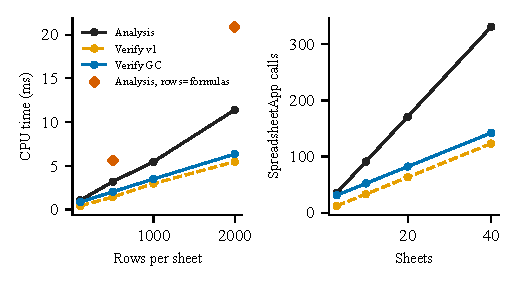
\includegraphics[width=\columnwidth]{figures/fig_e3_cost}
\caption{Cost of workbook analysis and of verifying one formula. Left: CPU time against rows per sheet (three sheets; diamonds: as many formulas as rows). Right: \code{SpreadsheetApp} calls against the number of sheets (500 rows per sheet). The data are those of Table~\ref{tab:e3}.}
\label{fig:e3-cost}
\end{figure}

\paragraph{SSRF corpus}
Table~\ref{tab:ssrf} lists the \ssrfBlock{} must-block and \ssrfAllow{} must-allow URLs by category. The shipped substring filter misses every decimal, hexadecimal, octal and otherwise encoded form of loopback and private addresses and every internal-only name, catches few IPv6-mapped and link-local addresses, and over-blocks benign URLs that contain a private-looking substring; the parse-and-classify validator is correct on all categories.

\begin{table}
\caption{SSRF corpus: URLs handled correctly (blocked if $\ast$, allowed otherwise) by the shipped substring filter (v1) and the parse-and-classify validator (v2).}
\label{tab:ssrf}

\centering\footnotesize
\begin{adjustbox}{max width=\columnwidth}\begin{tabular}{l r rr}
\toprule
\textbf{Category} & \textbf{n} & \textbf{v1} & \textbf{v2} \\
\midrule
$\ast$ loopback (dotted) & 6 & 2 & \textbf{6} \\
$\ast$ loopback (decimal/hex/octal) & 8 & 0 & \textbf{8} \\
$\ast$ loopback (IPv6) & 7 & 3 & \textbf{7} \\
$\ast$ unspecified & 4 & 3 & \textbf{4} \\
$\ast$ localhost names & 5 & 5 & \textbf{5} \\
$\ast$ private v4 (dotted) & 7 & 7 & \textbf{7} \\
$\ast$ private v4 (encoded) & 7 & 0 & \textbf{7} \\
$\ast$ link-local / metadata & 12 & 4 & \textbf{12} \\
$\ast$ IPv6-mapped / translated private & 6 & 2 & \textbf{6} \\
$\ast$ userinfo / authority tricks & 6 & 6 & \textbf{6} \\
$\ast$ wildcard-DNS names for private IPs & 6 & 3 & \textbf{6} \\
$\ast$ internal-only names & 6 & 0 & \textbf{6} \\
$\ast$ non-http schemes & 6 & 6 & \textbf{6} \\
$\ast$ unicode / formatting & 6 & 3 & \textbf{6} \\
public hosts & 8 & 8 & \textbf{8} \\
public IPs & 5 & 5 & \textbf{5} \\
boundary public addresses & 12 & 12 & \textbf{12} \\
public IPs with private-looking digits & 7 & 4 & \textbf{7} \\
benign URLs with suspicious substrings & 12 & 4 & \textbf{12} \\
IDN / unusual but public & 4 & 4 & \textbf{4} \\
\bottomrule
\end{tabular}\end{adjustbox}
\end{table}


\paragraph{Retrieval by budget}
Figure~\ref{fig:e2} shows gold-table completeness as the budget grows and Table~\ref{tab:e2} breaks down the 40-table setting by method. The seven-signal ranker is ahead of BM25 at every budget below that of the whole workbook; removing the lexical signal costs more than removing the graph signals.

\begin{figure}[!t]
\centering
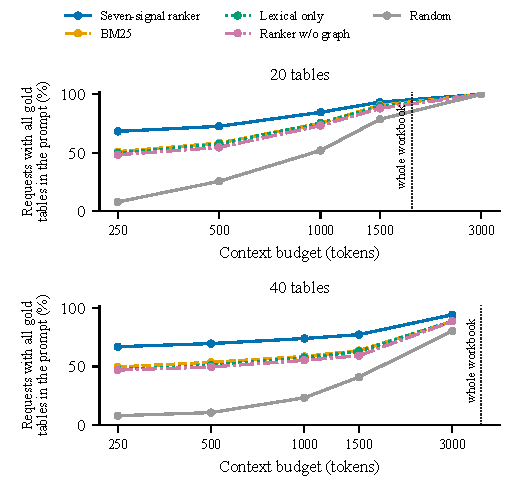
\includegraphics[width=\columnwidth]{figures/fig_e2_budget}
\caption{Share of requests whose prompt contains every gold table, by context budget, for workbooks with 20 and 40 tables. Dotted line: size of the whole workbook.}
\label{fig:e2}
\end{figure}

\begin{table}
\caption{Context retrieval on workbooks with 40 tables (300 requests). \emph{Complete}: share of requests whose prompt contains \emph{all} gold tables (\%); \emph{Recall}: mean fraction of gold tables retrieved (\%); \emph{Tokens}: mean prompt tokens spent on context.}
\label{tab:e2}

\centering\footnotesize
\begin{adjustbox}{max width=\columnwidth}\begin{tabular}{l rrr rrr}
\toprule
& \multicolumn{3}{c}{\textbf{Budget 1500}} & \multicolumn{3}{c}{\textbf{Budget 500}} \\
\cmidrule(lr){2-4}\cmidrule(lr){5-7}
\textbf{Method} & Complete & Recall & Tokens & Complete & Recall & Tokens \\
\midrule
Seven-signal ranker (shipped) & \textbf{77.3} & 77.3 & 1{,}488 & 69.7 & 69.7 & 487 \\
BM25 & 63.7 & 63.7 & 1{,}489 & 53.7 & 53.7 & 488 \\
Lexical (Jaccard) only & 63.0 & 63.0 & 1{,}488 & 51.0 & 51.0 & 487 \\
Ranker without graph signals & 59.3 & 59.3 & 1{,}488 & 49.7 & 49.7 & 488 \\
Ranker without lexical signal & 51.3 & 51.3 & 1{,}492 & 33.3 & 33.3 & 490 \\
Random & 41.0 & 41.0 & 1{,}487 & 10.7 & 10.7 & 490 \\
Active sheet only (as shipped to the agent) & 0.0 & 0.0 & 42 & 0.0 & 0.0 & 42 \\
Everything (no budget) & 100.0 & 100.0 & 3{,}723 & 100.0 & 100.0 & 3{,}723 \\
\bottomrule
\end{tabular}\end{adjustbox}
\end{table}


\paragraph{End-to-end study}
Table~\ref{tab:e5-taxonomy} gives the counts behind Figure~\ref{fig:e5-taxonomy}, and Table~\ref{tab:e5-repair-shipped} repeats the repair comparison with the chunk format the add-on shipped. Figure~\ref{fig:e5-templates} shows attempt-1 accuracy for every task template and model; the templates the local models fail are those that need a cross-sheet reference, a ranking or a conditional average. Table~\ref{tab:e5-cost} gives the generation cost.

\begin{table}
\caption{What verification sees among the formulas the model got wrong on its first attempt (final system). Flagged = rejected or warned.}
\label{tab:e5-taxonomy}

\centering\footnotesize
\begin{adjustbox}{max width=\columnwidth}\begin{tabular}{l rrrrrr}
\toprule
\textbf{Wrong at attempt 1} & \textbf{\shortstack[r]{Llama~3.1\\8B}} & \textbf{\shortstack[r]{Llama~3.2\\3B}} & \textbf{\shortstack[r]{Llama~3.1 8B\\new tasks}} & \textbf{\shortstack[r]{Gemini~3.1\\Flash-Lite}} & \textbf{\shortstack[r]{Gemini~3.5\\Flash-Lite}} & \textbf{\shortstack[r]{Gemma~4\\26B-A4B}} \\
\midrule
Wrong formulas & 105 & 220 & 50 & 8 & 12 & 15 \\
~~loud (engine error) & 67 & 110 & 29 & 1 & 3 & 4 \\
~~silent (wrong value) & 38 & 110 & 21 & 7 & 9 & 11 \\
Rejected by shipped verifier & 29 & 29 & 8 & 0 & 0 & 0 \\
Rejected by GroundCheck & 35 & 49 & 11 & 0 & 1 & 0 \\
Flagged by GroundCheck & 50 & 88 & 19 & 0 & 1 & 0 \\
Correct formulas rejected & 0/255 & 0/140 & 0/130 & 0/233 & 0/236 & 0/345 \\
\bottomrule
\end{tabular}\end{adjustbox}
\end{table}


\begin{table}
\caption{The repair comparison of Table~\ref{tab:e5-repair} repeated with retrieved context in the chunk format the add-on shipped (no column letters), forked from that arm's attempt 1.}
\label{tab:e5-repair-shipped}

\centering\footnotesize
\begin{adjustbox}{max width=\columnwidth}\begin{tabular}{l rr}
\toprule
& \multicolumn{2}{c}{\textbf{Llama~3.1 8B} (n=360)} \\
\textbf{Condition} & Acc. & $p_{\text{rs}}$ \\
\midrule
Attempt 1 & 64.4 & -- \\
Resample (no feedback) & 65.0 & -- \\
Generic feedback & 66.4 & .125 \\
Shipped-verifier feedback & 69.2 & <.001 \\
GroundCheck feedback & 70.3 & <.001 \\
GroundCheck + suspicious & 73.1 & <.001 \\
\bottomrule
\end{tabular}\end{adjustbox}
\end{table}


\begin{figure}[!t]
\centering
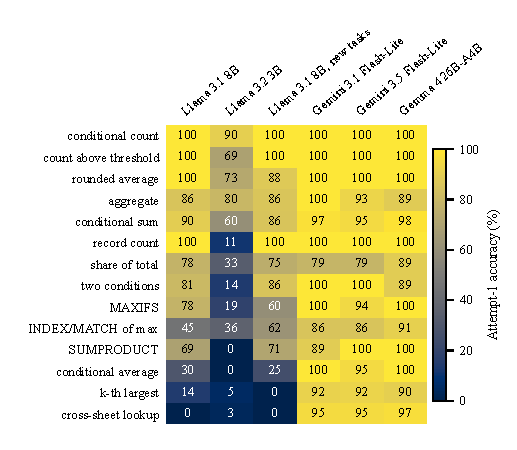
\includegraphics[width=\columnwidth]{figures/fig_e5_templates}
\caption{Attempt-1 accuracy with retrieved context by task template (rows) and model (columns); each cell is 11 to 58 tasks on the main set, 7 to 29 on the held-out set and at most 39 for each hosted model.}
\label{fig:e5-templates}
\end{figure}

\begin{table}
\caption{Generation cost per task by model: prompt tokens with the shipped active-sheet context and with retrieved context, wall-clock seconds for the first attempt (local models on one consumer GPU; hosted model over the network), and the extra model calls and seconds that repair with \gc{} feedback adds (--: not recorded in that pass).}
\label{tab:e5-cost}

\centering\footnotesize
\begin{adjustbox}{max width=\columnwidth}\begin{tabular}{l rrrrrr}
\toprule
\textbf{Per task} & \textbf{\shortstack[r]{Llama~3.1\\8B}} & \textbf{\shortstack[r]{Llama~3.2\\3B}} & \textbf{\shortstack[r]{Llama~3.1 8B\\new tasks}} & \textbf{\shortstack[r]{Gemini~3.1\\Flash-Lite}} & \textbf{\shortstack[r]{Gemini~3.5\\Flash-Lite}} & \textbf{\shortstack[r]{Gemma~4\\26B-A4B}} \\
\midrule
Prompt tokens, active sheet only & -- & 564 & 554 & 615 & 616 & 617 \\
Prompt tokens, retrieved context & 942 & 952 & 944 & 1{,}049 & 1{,}049 & 1{,}050 \\
Seconds, attempt 1 & 2.7 & 0.9 & 2.6 & 3.3 & 1.1 & 6.2 \\
Extra calls, \gc{} feedback & 0.13 & 0.21 & 0.10 & 0.00 & 0.00 & 0.00 \\
Extra seconds, \gc{} feedback & 0.4 & 0.2 & 0.3 & 0.0 & 0.0 & 0.0 \\
\bottomrule
\end{tabular}\end{adjustbox}
\end{table}


\section{Checking the labels in Google Sheets}
\label{app:gsheets}

The labels of \sheetfault{} come from HyperFormula, which follows Excel, while the system targets Google Sheets. To check that the labels carry over, the repository holds a validation harness: a stratified sample of \gsPackCases{} benchmark cases over \gsPackWorkbooks{} workbooks (\gsPackPerFault{} per fault class, \gsPackPerClean{} per clean class), an Apps Script that builds each case's workbook in a Google Sheet, puts the formula in the target cell and records what the cell shows, and a script that compares the two engines' answers case by case and re-derives the faulty/clean label under Google Sheets. The harness stops and resumes within the Apps Script time limit. Its control flow, resumption and comparison were tested against a mock of the Apps Script services backed by HyperFormula, on which all cases agree, as they must; that test says nothing about Google Sheets.

\ifdefined\gsN
Run in Google Sheets, the two engines give the same answer (an error in both, or the same value) for \gsSame\% of the \gsN{} cases: HyperFormula errs where Sheets does not in \gsHfErrOnly{}, Sheets errs where HyperFormula does not in \gsGsErrOnly{}, and the values differ in \gsDiffValues{}. The faulty/clean label is identical under both engines for \gsLabelSame\% of the cases (\gsFlipFault{} faulty under HyperFormula only, \gsFlipClean{} faulty under Sheets only). On the sampled faults \gc{} rejects \gsvtwoRecallHF\% under HyperFormula labels and \gsvtwoRecallGS\% under Google Sheets labels (shipped verifier: \gsvoneRecallHF\% and \gsvoneRecallGS\%), and rejects \gsvtwoFPRGS\% of the clean cases under Sheets labels.
\else
The run in Google Sheets is not part of this version of the paper, so every label here is a HyperFormula label. The harness reports the same quantities as the benchmark tables, so a run adds one paragraph to this appendix.
\fi

\section{Independent annotation of real formulas}
\label{app:annotation}

The real-formula sets have no labels (Section~\ref{sec:rwmethod}). The repository holds a protocol and tooling for blind annotation: a sample of 400 confirmation-set formulas stratified by the verifiers' decisions (\gc{} rejects, \gc{} only warns, only the shipped verifier rejects, both accept), shuffled and stripped of all verifier output, with the formula, its workbook's sheet names and sizes, the neighbourhood of the target cell and the sheets the formula names; written guidelines (defect Y/N/U, loud or silent, a category); a scorer that reports agreement between two annotators (raw and Cohen's $\kappa$), takes adjudicated labels for disagreements, and reports weighted precision, recall and false-positive rate of each verifier with workbook-clustered intervals. The tooling was tested on synthetic annotations only.

\ifdefined\annN
Two annotators labelled \annOf{} formulas independently; they agreed on \annAgree\% (Cohen's $\kappa$ \annKappa{}; \annKappaYN{} for defect against no defect) and settled \annDisagree{} disagreements together, leaving \annN{} formulas scored. Weighted back to the population, \annPrevalence\% of formulas are defective. On this ground truth the shipped verifier's rejections have precision \annVoneP\% [\annVonePLo, \annVonePHi] and recall \annVoneR\% [\annVoneRLo, \annVoneRHi]; \gc's have precision \annVtwoP\% [\annVtwoPLo, \annVtwoPHi] and recall \annVtwoR\% [\annVtwoRLo, \annVtwoRHi], with false-positive rates of \annVoneF\% and \annVtwoF\%.
\else
No annotation is part of this version: the numbers of Section~\ref{sec:e1b} are rejection rates, with an engine's evaluation as supporting evidence, and we claim no precision or recall on real formulas.
\fi
